\begin{frame}{Was sind kosmische Phasenübergänge?}
   \begin{columns}
 \begin{column}{0.9\textwidth}
  \begin{itemize}
    \item  GUT, die Vereinigung aller Kräfte
    \item  Bildung stabiler Teilchen
    \item  Bildung stabiler Kerne
    \item  Durchlässigkeit des Plasma's für elektromagnetische Strahlung
  \end{itemize}
\begin{figure}
  \centering
  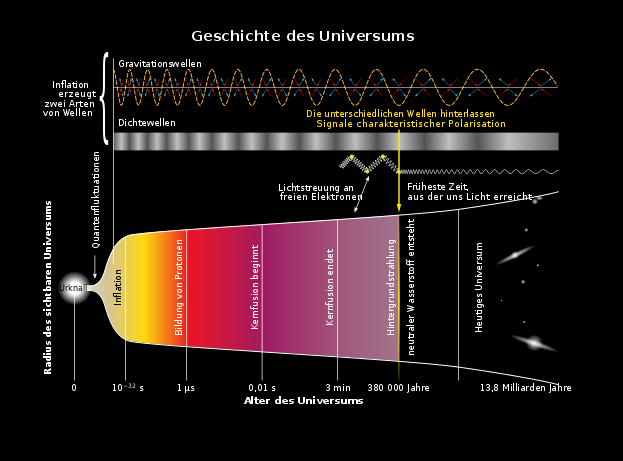
\includegraphics[width=0.55\textwidth]{images/Frage1.PNG}
\end{figure}
\end{column}
\end{columns}
\end{frame}


\begin{frame}{Wiederholt sich das Universum immer wieder?}
Empirisch nicht nachweisbar!
\end{frame}


\begin{frame}{Wie stellt man sich Dunkle Materie vor?}
  \begin{itemize}
    \setlength\itemsep{2em}
    \item Ähnlich wie Neutrinos
    \item Neutrinos haben kaum Wechselwirkung mit Materie (aber immer
    gravitativ)
    \item Dunkle Materie wechselwirkt nur gravitativ
    \item  Viele Theorien (Neutralinos (Eigenes Antiteilchen) etc.),
    aber bis heute keine sicheren Ergebnisse.
  \end{itemize}
\end{frame}

\begin{frame}{Gibt es Antiteilchen für Eichbosonen?}

$W^+$ ist Antiteilchen zu $W^-$, $\gamma$ und $Z^0$ sind ihr eigenes Antiteilchen.

\vspace{0.5cm}

\begin{columns}[T, onlytextwidth]
  \begin{column}{0.47\textwidth}
    \begin{itemize}
      \setlength\itemsep{2em}
      \item Gibt es Wurmlöcher? Ist deren Existenz vorstellbar, wenn ja, wie funktioniert dies? \\
      $\longrightarrow$ Bis heute keins nachgewiesen, vorstellbar ja.
    \end{itemize}
  \end{column}
  \hfill
  \begin{column}{0.47\textwidth}
    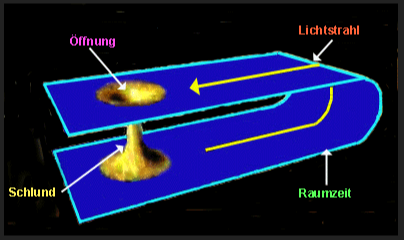
\includegraphics[width=\textwidth]{images/Frage2.PNG}
  \end{column}
\end{columns}


\end{frame}

\begin{frame}{AGN's}
\begin{itemize}
  \setlength\itemsep{2em}
  \item Wie genau kann man sich ein flaches bzw. gekrümmtes Universum vorstellen?
  $\longrightarrow$ Gar nicht. Es ist nur indirekt beobachtbar.
  \item Wodurch genau sind die AGNs gekennzeichnet?
  $\longrightarrow$ AGN = Active Galactic Nuclei, also in der Mitte einer Galaxie.
  $\longrightarrow$ Da nur Massen Massen anziehen ist im Prinzip das gesamte
  System Galaxie gravitativ an den Kern gebunden.
  $\longrightarrow$ Dort, wo so viel Masse ist, wird auch viel Strahlung
  ausgesendet. AGN's sind deshalb vergleichsweise sehr leuchtkräftige Objekte.
  \item Wie entstehen die Jets der AGNs?
  $\longrightarrow$ Drehimpulserhaltung
\end{itemize}
\end{frame}

\begin{frame}{Gravitation}
\begin{itemize}
  \setlength\itemsep{2em}
  \item Woher stammt die Gravitation?
  $\longrightarrow$ Theorien: Higgs-Feld, Graviton
  \item Wie setzt sich die Masse der Elementarteilchen zusammen?
  $\longrightarrow$ Valenzquarks und Seequarks (Quark-Antiquark-Paare).
  \item Wie schafft es ein Neutronenstern den Fermidruck zu überwinden?
  $\longrightarrow$ Akkretion von Materie.
  \item Wie genau funktioniert der Gravitationslinseneffekt?
  $\longrightarrow$ Massen beeinflussen Photonen, also: Licht wird abgelenkt
\end{itemize}
\end{frame}

\begin{frame}{Schwarze Löcher}
  \begin{itemize}
    \setlength\itemsep{2em}
    \item Wieso gibt es für die Energiefreigabe im Universum (z.B. durch
    Kollision von schwarzen Löchern) eine Obergrenze? Es ist doch genügend
    Energie vorhanden, wie können unterschiedliche Ereignisse davon etwas
    mitbekommen?
   $\longrightarrow$ Gibt es nicht. Es werden einfach nur etwa drei Sonnenmassen
   Energie freigegeben bei der Fusion zweier schwarzer Löcher.
   \item Warum zeigt der Jet eines schwarzen Loches nach "oben"?
   Die Teilchen, die Drehimpuls durch andere Teilchen erhalten
   haben könnten sich doch auch in der Ebene von dem schwarzen Loch entfernen,
   warum nach "oben"?
   $\longrightarrow$ Missverständnis. Durch Gesetze der Physik
   (Drehimpulserhaltung, Gravitation usw.) ist es fest, wohin der Jet geht, aber
   nach "oben" geht er meistens in den Skizzen, die von schwarzen Löchern oder
   AGN's gemacht werden. Wenn wir einen Jet detektieren können, dann weil dessen
   Jet auf unsere Messgeräte gerichtet ist.
   \item Was passiert in der Nähe eines schwarzen Lochs?
   $\longrightarrow$ Masse wird akkretiert
   $\longrightarrow$ Ereignishorizont
   $\longrightarrow$ Strukturbildungen, die den Regeln der Gravitation folgen
\end{itemize}

\end{frame}

\begin{frame}
  \begin{itemize}
    \setlength\itemsep{2em}
    \item In der Nähe eines schwarzen Loches wirken ja starke Magnetfelder. Aber
    wie verhalten sich externe Magnetfelder anderer Quellen in der Nähe des
    schwarzen Loches? Folgen die Feldlinien dem gekrümmten Raum oder inwiefern
    werden sie verzerrt?
    $\longrightarrow$ Ja. Wie auch bei allen anderen Magneten
  \end{itemize}
\begin{figure}[H]
  \centering
  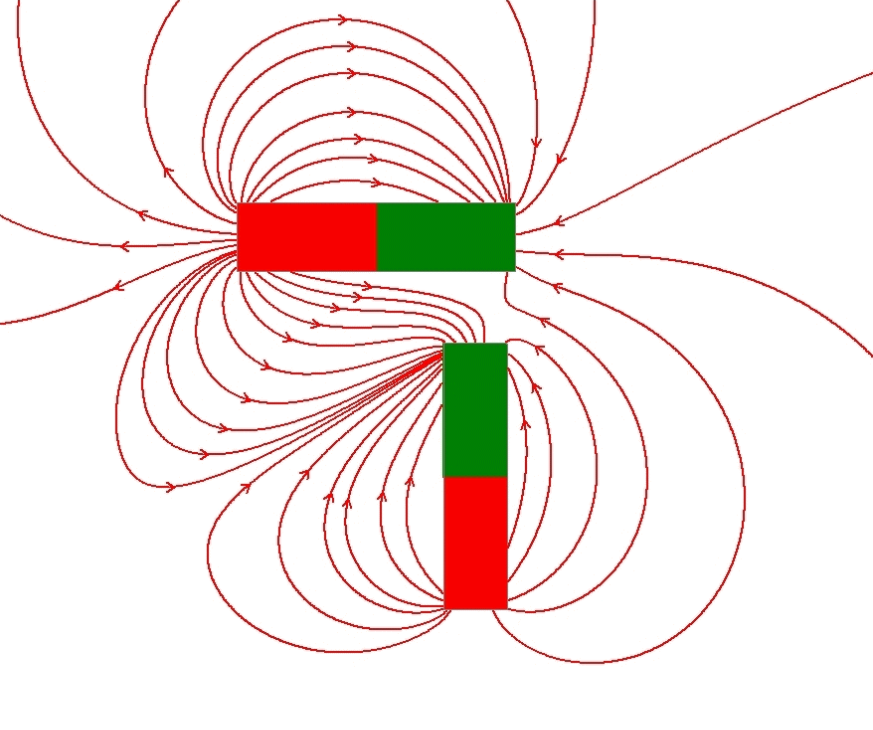
\includegraphics[width=0.5\textwidth]{images/Frage3.PNG}
  \caption{Magneten auf der Erde verhalten sich wie Magneten im Interstellaren Raum.}
\end{figure}
\end{frame}
